\documentclass[12pt]{beamer}
\usepackage{ucltemplate}


\usepackage{lineno,hyperref}
\usepackage{stfloats}
\usepackage{tikz} % Package for drawing
\usepackage{amsmath}
\usepackage{mathtools}
\usepackage{amsfonts}
\usepackage{float}
\usepackage{lmodern,bm}                
\usepackage[T1]{sansmath} 
\usepackage{amsthm}
\usepackage{url}
\usepackage[toc,page]{appendix}
\usepackage{graphicx}
\usepackage{subcaption}
\usepackage{verbatim} %to comment out sections
\usetikzlibrary{shapes.multipart}
\usetikzlibrary{matrix}
\usetikzlibrary{positioning}
\usepackage{float}
\usepackage{color}
\usepackage{booktabs}
\usepackage{placeins}
\usepackage{bm}
\usepackage[natbib=true,style=authoryear,backend=bibtex,useprefix=true]{biblatex}

\newcommand{\myfootnote}[1]{
    \renewcommand{\thefootnote}{}
    \footnotetext{\scriptsize#1}
    \renewcommand{\thefootnote}{\arabic{footnote}}
}
\setbeamerfont{footnote}{size=\tiny}
\addbibresource{bibliography.bib}

\newcommand{\curl}{\mathbf{curl}}
\newcommand{\divergence}{\textnormal{div}}
\DeclarePairedDelimiter\floor{\lfloor}{\rfloor}

\title{Fast Calder\'on preconditioning of the PMCHWT formulation for scattering by multiple dielectric objects}
\subtitle[The subtitle]{\tiny{$14^{th}$ International Conference on Mathematical and Numerical Aspects of Wave Propagation, Vienna, Austria}}
\author{\textbf{Antigoni Kleanthous} \inst{1},  Timo Betcke \inst{1}, David Hewett \inst{1}, Carlos Jerez-Hanckes \inst{2}, Paul Escapil-Inchausp\'e \inst{3}, Anthony J. Baran \inst{4,5}}
\institute{\inst{1} Department of Mathematics, UCL, UK  \\ \inst{2} Universidad Adolfo Iba\~nez, Santiago, Chile \\
\inst{3} Pontificia Universidad Cat\'olica de Chile, Santiago, Chile \\
\inst{4} Met Office, UK \\ \inst{5} School of Physics, Astronomy, and Mathematics, University of Hertfordshire, UK}
\date{30 August 2019}

\usepackage{pdfpages}

\begin{document}

% \begin{frame}
%   \titlepage
%   \vspace*{-1.8cm}
%   \flushright 
%   \includegraphics[height = 1.3cm]{Figures/nerc-logo_eps.pdf} 
%   \hspace*{0.2cm}
%   \includegraphics[height = 1.3cm]{Figures/met-logo.jpg}
% \end{frame}

\begin{frame}
\includepdf{Figures/title_slide.pdf}
\end{frame}

%%%
\begin{frame}{Introduction}
%\myfootnote{\fullcite{kleanthous2019calderon}} 
Plan
\begin{itemize}
\item The scattering problem
\item The Boundary Element Method
\item Preconditioning
\item Bempp and Bempp-cl: Boundary Element Software
\item Numerical Benchmarks
\item Application to aggregates
\end{itemize}
\end{frame}
%%%


%%%
\begin{frame}{The scattering problem}
\vspace{0.2cm}
\centering
    \includegraphics[width = \textwidth]{Figures/problem.png}
    
\vspace*{-0.5cm}    
\begin{footnotesize}    
\begin{itemize}
    \item $(\mathbf{E}^i_m, \mathbf{H}^i_m)$ and $(\mathbf{E}^e, \mathbf{H}^e)$: interior and exterior fields with
        \begin{alignat}{1}
            \mathbf{E}^e = \mathbf{E}^{inc} + \mathbf{E}^s, \quad 
            \mathbf{H}^e = \mathbf{H}^{inc} + \mathbf{H}^s, \nonumber
        \end{alignat}
    \item Time-harmonic Maxwell equations
    \begin{alignat}{3}
        \only<1>{\nabla \times \mathbf{E}^i_m &=& i \omega \mu_m \mathbf{H}^i_m, \quad \nabla \times \mathbf{H}^i_m &=& - i \omega \epsilon_m \mathbf{E}^i_m, &\qquad\text{in }\Omega^i_m, \nonumber \\
        \nabla \times \mathbf{E}^e &=& i \omega \mu_e \mathbf{H}^e, \quad \nabla \times \mathbf{H}^e &=& - i \omega \epsilon_e \mathbf{E}^e &\qquad\text{in }\Omega^e, \nonumber}
        \only<2>{&\nabla \times (\nabla \times \mathbf{E}^i_m) &-& k_m^2 \mathbf{E}^i_m &= 0,\qquad&\text{in }\Omega^i_m, \nonumber\\
        &\nabla \times (\nabla \times \mathbf{E}^e) &-& k_e^2 \mathbf{E}^e &= 0,\qquad&\text{in }\Omega^e, \nonumber} 
\end{alignat}
    \item Transmission boundary conditions
        \begin{alignat}{3}
            \only<1>{\mathbf{E}^i_m (\mathbf{x}) \times \mathbf{n} &= \mathbf{E}^e (\mathbf{x}) \times \mathbf{n}, \quad \mathbf{H}^i_m (\mathbf{x}) \times \mathbf{n} &= \mathbf{H}^e (\mathbf{x}) \times \mathbf{n}, && \quad \mathbf{x} \in \Gamma_m. \nonumber}
            \only<2>{\mathbf{E}^i_m (\mathbf{x}) \times \mathbf{n} &= \mathbf{E}^e (\mathbf{x}) \times \mathbf{n}, && \quad \mathbf{x} \in \Gamma_m. \nonumber}
\end{alignat}
\end{itemize}
\end{footnotesize}
\end{frame}
%%%
\begin{frame}{The Boundary Element Method}
\begin{itemize}
    \item reformulate the problem as boundary integral equations on the boundary $\Gamma$
    \pause
    \item solve the problem on the boundary
    \pause
    \item extend the solution to the domain of interest (e.g. interior/exterior of scatterer) via representation formulae
\end{itemize}
\end{frame}
%%%

%%%
\begin{frame}{Why the Boundary Element Method}
\myfootnote{\fullcite{baran2012single}}
\begin{itemize}
    \item lower dimensional manifold to discretise
    \pause
    \item automatically incorporates outgoing behaviour at infinity
    \pause
    \item flexibility with geometry; it can handle complex domains such as ice crystals
\end{itemize}
\begin{figure}
    \centering
    \includegraphics[width = 0.3 \textwidth]{Figures/ice_crystals.png}
    \caption{Ice Models. Taken from (Baran, 2012). }
\end{figure}
    
\end{frame}

%%%
\begin{frame}{Boundary Integral Operators}
\begin{footnotesize}
    \begin{itemize}
        \item Electric and Magnetic Potential Operators
            \begin{alignat}{2}
                &\mathcal{E} \mathbf{v}(\mathbf{x}) &:=& ik \int _{\Gamma} \mathbf{v}(\mathbf{y}) G (\mathbf{x}, \mathbf{y}) d \Gamma (\mathbf{y}) - \frac{1}{ik} \nabla_\mathbf{x} \int _\Gamma \nabla_\mathbf{y} \cdot \mathbf{v}(\mathbf{y}) G (\mathbf{x}, \mathbf{y}) d\Gamma (\mathbf{y}), \nonumber\\
                %
                &\mathcal{H} \mathbf{v}(\mathbf{x}) &:=& \nabla_\mathbf{x} \times \int _\Gamma \mathbf{v}(\mathbf{y}) G (\mathbf{x}, \mathbf{y}) d \Gamma (\mathbf{y}), \nonumber 
            \end{alignat}
            where $G (x,y) = \frac{\exp (ik | \mathbf{x} - \mathbf{y}|)}{4 \pi | \mathbf{x} - \mathbf{y}|}$
        \item Dirichlet and Neumann Traces
            \begin{alignat}{3}
                \gamma_{D}^{\pm} \mathbf{u} (\mathbf{x}) &:= \mathbf{u}(\mathbf{x}) \times \mathbf{n}, \quad 
                \gamma_{N}^{\pm} \mathbf{u}(\mathbf{x}) &:= \frac{1}{ik} \gamma_{D}^{\pm} \left( \nabla \times \mathbf{u}(\mathbf{x}) \right), \quad &\mathbf{x} \in \Gamma \nonumber 
            \end{alignat}
        \item Boundary Integral Operators
            \begin{alignat}{3}
                &\mathcal{S} &:=& \{ \gamma_D \}\mathcal{E} &=& -\{ \gamma_{N} \} \mathcal{H}, \nonumber \\
                &\mathcal{C} &:=& \{ \gamma _{D} \} \mathcal{H} &=& \{ \gamma _{N} \} \mathcal{E}, \nonumber 
            \end{alignat}
    \end{itemize}
\end{footnotesize}
\end{frame}
%%%

%%%
\begin{frame}{Boundary Integral Operators}
\begin{footnotesize}
\begin{itemize}
    \item Stratton Chu Representation Formulae
        \begin{alignat}{3}
            \mathcal{H}^i_m (\gamma_{D,m}^- \mathbf{E}^i_m) &+ \mathcal{E}^i_m (\gamma_{N,m}^- \mathbf{E}^i_m) &= 
            \begin{cases}
                \mathbf{E}^i_m(\mathbf{x}), & \mathbf{x} \in \Omega^i_m, \\
                \mathbf{0}, & \mathbf{x} \not \in \overline{\Omega^i_m},
            \end{cases} \nonumber\\
            %
            -\sum_m^M \mathcal{H}^e_m (\gamma_{D,m}^+ \mathbf{E}^s) &- \sum_m^M  \mathcal{E}^e_m (\gamma_{N,m}^+ \mathbf{E}^s) &= 
            \begin{cases}
                \mathbf{E}^s(\mathbf{x}), & \mathbf{x} \in \Omega_e, \\
                \mathbf{0}, & \mathbf{x} \not \in \overline{\Omega_e},
            \end{cases} \nonumber 
        \end{alignat}
\end{itemize}
\end{footnotesize}    
\end{frame}
%%%

% %%%
% \begin{frame}{Boundary Integral Operators}
% \begin{footnotesize}
% Taking appropriate interior and exterior Dirichlet and Neumann traces of the Stratton Chu representation formulae
% \begin{align}
% &\left( \frac{1}{2}\bm{\mathcal{I}}_m - \bm{\mathcal{{A}}}^i_m \right){\mathbf{u}}^i_m = 0, \nonumber\\
% &\left( \frac{1}{2} \bm{\mathcal{I}}_m + \bm{\mathcal{{A}}}^e_m \right) {\mathbf{u}}^s_m + \sum _{\ell \neq m}^M \bm{\mathcal{{A}}}_{m\ell} {\mathbf{u}}^s_\ell= 0 , \nonumber 
% \end{align}
% where
% \begin{gather}
% \bm{\mathcal{{A}}}^i_m = \begin{bmatrix}
% \mathcal{C}^i_m & \frac{\mu_m}{k_m} \mathcal{S}^i_m \\[6pt]
% -\frac{k_m}{\mu_m} \mathcal{S}^i_m & \mathcal{C}^i_m
% \end{bmatrix}, \quad 
% \bm{\mathcal{{A}}}^e_m = \begin{bmatrix}
% \mathcal{C}^e_m & \frac{\mu_e}{k_e} \mathcal{S}^e_m \\[6pt]
% -\frac{k_e}{\mu_e} \mathcal{S}^e_m & \mathcal{C}^e_m
% \end{bmatrix}, \nonumber \\
% \bm{\mathcal{{A}}}_{m\ell} = \begin{bmatrix}
%     \mathcal{C}^e_{m\ell} & \frac{\mu_e}{k_e} \mathcal{S}^e_{m\ell} \\[6pt]
%     -\frac{k_e}{\mu_e} \mathcal{S}^e_{m\ell} & \mathcal{C}^e_{m\ell}
% \end{bmatrix}, \quad
% %
% {\mathbf{u}}^i_m = \begin{bmatrix}
%     \gamma_{D,m}^{-} \mathbf{E}^i_m \\[6pt]
%     \frac{k_m}{\mu_m} \gamma_{N,m}^- \mathbf{E}^i_m
% \end{bmatrix}, \quad 
% %
% {\mathbf{u}}^s_m = \begin{bmatrix}
%     \gamma_{D,m}^+ \mathbf{E}^s \\[6pt]
%     \frac{k_e}{\mu_e} \gamma_{N,m}^+ \mathbf{E}^s
% \end{bmatrix} \nonumber .
% \end{gather}
% \end{footnotesize}    
% \end{frame}
% %%%

% %%%
% \begin{frame}{The PMCHWT formulation}
% \begin{footnotesize}
% Combine
% \begin{align}
% &\left( \frac{1}{2}\bm{\mathcal{I}}_m - \bm{\mathcal{{A}}}^i_m \right){\mathbf{u}}^i_m = 0, \nonumber\\
% &\left( \frac{1}{2} \bm{\mathcal{I}}_m + \bm{\mathcal{{A}}}^e_m \right) {\mathbf{u}}^s_m + \sum _{\ell \neq m}^M \bm{\mathcal{{A}}}_{m\ell} {\mathbf{u}}^s_\ell= 0 , \nonumber 
% \end{align}
% with transmission conditions
% \begin{alignat}{3}
% {\mathbf{u}}^i_m = {\mathbf{u}}^s_m + {\mathbf{u}}^{inc}_m,\quad m=1,\ldots, M, \nonumber
% \end{alignat}
% to get the PMCHWT formulation for each $m$
% \begin{alignat}{1}
% \left(\bm{\mathcal{{A}}}^i_m + \bm{\mathcal{{A}}}^e_m\right) {\mathbf{u}}^s_m + \sum _{\ell \neq m}^j \bm{\mathcal{{A}}}_{m\ell} {\mathbf{u}}^s_\ell = \left( \frac{1}{2}\bm{\mathcal{I}} - \bm{\mathcal{{A}}}^i_m \right) {\mathbf{u}}^{inc}_m. \nonumber 
% \end{alignat}
% \end{footnotesize}    
% \end{frame}
% %%%

% %%%
% \begin{frame}{The PMCHWT formulation}
% \begin{alignat}{3}
% \bm{\mathcal{A}}\mathbf{ u}^s = \left(\frac{1}{2}\bm{\mathcal{ {I}}} - \bm{\mathcal{{A}}}^i \right) \mathbf{u}^{inc} \nonumber 
% \end{alignat}
% % 
% \pause
% \begin{scriptsize}
% \begin{align}
% &\bm{\mathcal{A}} &=& 
% \begin{tikzpicture}[baseline={([yshift=-.5ex]current bounding box.center)}, ampersand replacement=\&]
% \matrix (m) [matrix of math nodes,nodes in empty cells,right delimiter={]},left delimiter={[} ]{
% \bm{\mathcal{{A}}}^e_1+\bm{\mathcal{{A}}}^i_1  \& \bm{\mathcal{{A}}}_{12}   \& \cdots  \& \bm{\mathcal{{A}}}_{1M}  \\
% \bm{\mathcal{{A}}}_{21}    \& \& \& \vdots \\
% \vdots  \&   \& \& \bm{\mathcal{{A}}}_{(M-1)M}   \\
% \bm{\mathcal{{A}}}_{M1}  \& \cdots  \& \bm{\mathcal{{A}}}_{M(M-1)}   \& \bm{\mathcal{{A}}}^e_M+\bm{\mathcal{{A}}}^i_M\\
% } ;
% \draw[loosely dotted,thick] (m-1-1)-- (m-4-4);
% \draw[loosely dotted,thick] (m-1-2)-- (m-3-4);
% \draw[loosely dotted,thick] (m-2-1)-- (m-4-3);
% \end{tikzpicture},  
% \bm{\mathcal{A}}^i = 
% \begin{tikzpicture}[baseline={([yshift=-.5ex]current bounding box.center)}, ampersand replacement=\&]
% \matrix (m) [matrix of math nodes,nodes in empty cells,right delimiter={]},left delimiter={[} ]{
% \bm{\mathcal{{A}}}^i_1  \& 0   \& \cdots  \& 0  \\
% 0    \& \& \& \vdots \\
% \vdots  \&   \& \& 0   \\
% 0 \& \cdots  \& 0 \& \bm{\mathcal{{A}}}^i_M\\
% } ;
% \draw[loosely dotted,thick] (m-1-1)-- (m-4-4);
% \draw[loosely dotted,thick] (m-1-2)-- (m-3-4);
% \draw[loosely dotted,thick] (m-2-1)-- (m-4-3);
% \end{tikzpicture}, \nonumber\\
% &\bm{\mathcal{I}} &=& 
% \begin{tikzpicture}[baseline={([yshift=-.5ex]current bounding box.center)}, ampersand replacement=\&]
% \matrix (m) [matrix of math nodes,nodes in empty cells,right delimiter={]},left delimiter={[} ]{
% \bm{\mathcal{{I}}}_1  \& 0   \& \cdots  \& 0  \\
% 0    \& \& \& \vdots \\
% \vdots  \&   \& \& 0   \\
% 0 \& \cdots  \& 0 \& \bm{\mathcal{{I}}}_M\\
% } ;
% \draw[loosely dotted,thick] (m-1-1)-- (m-4-4);
% \draw[loosely dotted,thick] (m-1-2)-- (m-3-4);
% \draw[loosely dotted,thick] (m-2-1)-- (m-4-3);
% \end{tikzpicture},  \quad 
% \mathbf{u}^s = 
% \begin{tikzpicture}[baseline={([yshift=-.5ex]current bounding box.center)}, ampersand replacement=\&]
% \matrix (m) [matrix of math nodes,nodes in empty cells,right delimiter={]},left delimiter={[} ]{
% {\mathbf{u}}^s_1    \\
% {\mathbf{u}}^s_2  \\
% \vdots   \\
% {\mathbf{u}}^s_M\\
% };
% \end{tikzpicture},  \quad
% \mathbf{u}^{inc} = 
% \begin{tikzpicture}[baseline={([yshift=-.5ex]current bounding box.center)}, ampersand replacement=\&]
% \matrix (m) [matrix of math nodes,nodes in empty cells,right delimiter={]},left delimiter={[} ]{
% {\mathbf{u}}^{inc}_1    \\
% {\mathbf{u}}^{inc}_2  \\
% \vdots   \\
% {\mathbf{u}}^{inc}_M\\
% }; \nonumber   
% \end{tikzpicture}.
% \end{align}
% \end{scriptsize}
% \end{frame}
% %%%

%%%
\begin{frame}{The PMCHWT formulation}
\begin{alignat}{3}
\bm{\mathcal{A}}\mathbf{ u}^s = \left(\frac{1}{2}\bm{\mathcal{ {I}}} - \bm{\mathcal{{A}}}^i \right) \mathbf{u}^{inc} \nonumber 
\end{alignat}
% 
\pause
\begin{scriptsize}
\begin{align}
&\bm{\mathcal{A}} &=& 
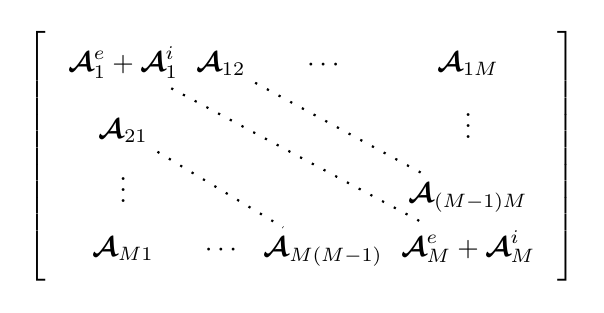
\begin{tikzpicture}[baseline={([yshift=-.5ex]current bounding box.center)}, ampersand replacement=\&]
\matrix (m) [matrix of math nodes,nodes in empty cells,right delimiter={]},left delimiter={[} ]{
\bm{\mathcal{{A}}}^e_1+\bm{\mathcal{{A}}}^i_1  \& \bm{\mathcal{{A}}}_{12}   \& \cdots  \& \bm{\mathcal{{A}}}_{1M}  \\
\bm{\mathcal{{A}}}_{21}    \& \& \& \vdots \\
\vdots  \&   \& \& \bm{\mathcal{{A}}}_{(M-1)M}   \\
\bm{\mathcal{{A}}}_{M1}  \& \cdots  \& \bm{\mathcal{{A}}}_{M(M-1)}   \& \bm{\mathcal{{A}}}^e_M+\bm{\mathcal{{A}}}^i_M\\
} ;
\draw[loosely dotted,thick] (m-1-1)-- (m-4-4);
\draw[loosely dotted,thick] (m-1-2)-- (m-3-4);
\draw[loosely dotted,thick] (m-2-1)-- (m-4-3);
\end{tikzpicture},  
\bm{\mathcal{A}}^i = 
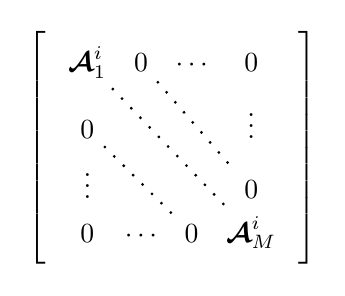
\begin{tikzpicture}[baseline={([yshift=-.5ex]current bounding box.center)}, ampersand replacement=\&]
\matrix (m) [matrix of math nodes,nodes in empty cells,right delimiter={]},left delimiter={[} ]{
\bm{\mathcal{{A}}}^i_1  \& 0   \& \cdots  \& 0  \\
0    \& \& \& \vdots \\
\vdots  \&   \& \& 0   \\
0 \& \cdots  \& 0 \& \bm{\mathcal{{A}}}^i_M\\
} ;
\draw[loosely dotted,thick] (m-1-1)-- (m-4-4);
\draw[loosely dotted,thick] (m-1-2)-- (m-3-4);
\draw[loosely dotted,thick] (m-2-1)-- (m-4-3);
\end{tikzpicture}, \nonumber\\
&\bm{\mathcal{I}} &=& 
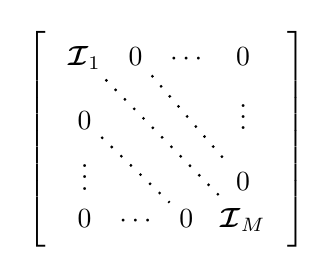
\begin{tikzpicture}[baseline={([yshift=-.5ex]current bounding box.center)}, ampersand replacement=\&]
\matrix (m) [matrix of math nodes,nodes in empty cells,right delimiter={]},left delimiter={[} ]{
\bm{\mathcal{{I}}}_1  \& 0   \& \cdots  \& 0  \\
0    \& \& \& \vdots \\
\vdots  \&   \& \& 0   \\
0 \& \cdots  \& 0 \& \bm{\mathcal{{I}}}_M\\
} ;
\draw[loosely dotted,thick] (m-1-1)-- (m-4-4);
\draw[loosely dotted,thick] (m-1-2)-- (m-3-4);
\draw[loosely dotted,thick] (m-2-1)-- (m-4-3);
\end{tikzpicture},  \quad 
\mathbf{u}^s = 
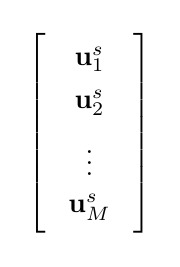
\begin{tikzpicture}[baseline={([yshift=-.5ex]current bounding box.center)}, ampersand replacement=\&]
\matrix (m) [matrix of math nodes,nodes in empty cells,right delimiter={]},left delimiter={[} ]{
{\mathbf{u}}^s_1    \\
{\mathbf{u}}^s_2  \\
\vdots   \\
{\mathbf{u}}^s_M\\
};
\end{tikzpicture},  \quad
\mathbf{u}^{inc} = 
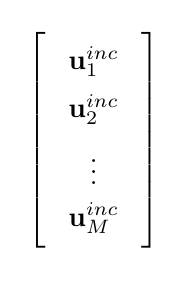
\begin{tikzpicture}[baseline={([yshift=-.5ex]current bounding box.center)}, ampersand replacement=\&]
\matrix (m) [matrix of math nodes,nodes in empty cells,right delimiter={]},left delimiter={[} ]{
{\mathbf{u}}^{inc}_1    \\
{\mathbf{u}}^{inc}_2  \\
\vdots   \\
{\mathbf{u}}^{inc}_M\\
}; \nonumber   
\end{tikzpicture}.
\end{align}
\end{scriptsize}
\end{frame}
%%%

%%%%
\begin{frame}{The PMCHWT formulation}
\begin{scriptsize}
\begin{align}
&\bm{\mathcal{A}} &=& 
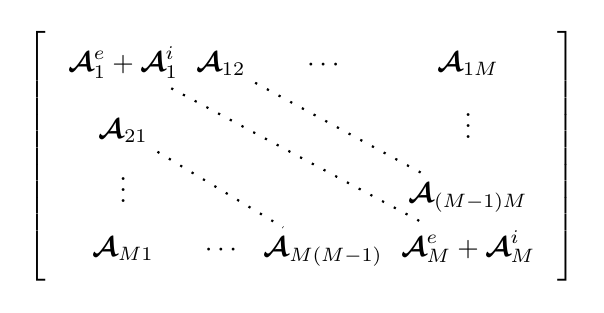
\begin{tikzpicture}[baseline={([yshift=-.5ex]current bounding box.center)}, ampersand replacement=\&]
\matrix (m) [matrix of math nodes,nodes in empty cells,right delimiter={]},left delimiter={[} ]{
\bm{\mathcal{{A}}}^e_1+\bm{\mathcal{{A}}}^i_1  \& \bm{\mathcal{{A}}}_{12}   \& \cdots  \& \bm{\mathcal{{A}}}_{1M}  \\
\bm{\mathcal{{A}}}_{21}    \& \& \& \vdots \\
\vdots  \&   \& \& \bm{\mathcal{{A}}}_{(M-1)M}   \\
\bm{\mathcal{{A}}}_{M1}  \& \cdots  \& \bm{\mathcal{{A}}}_{M(M-1)}   \& \bm{\mathcal{{A}}}^e_M+\bm{\mathcal{{A}}}^i_M\\
} ;
\draw[loosely dotted,thick] (m-1-1)-- (m-4-4);
\draw[loosely dotted,thick] (m-1-2)-- (m-3-4);
\draw[loosely dotted,thick] (m-2-1)-- (m-4-3);
\end{tikzpicture},   
\mathbf{u}^s = 
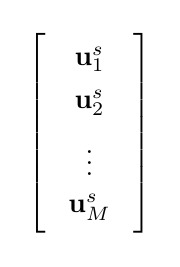
\begin{tikzpicture}[baseline={([yshift=-.5ex]current bounding box.center)}, ampersand replacement=\&]
\matrix (m) [matrix of math nodes,nodes in empty cells,right delimiter={]},left delimiter={[} ]{
{\mathbf{u}}^s_1    \\
{\mathbf{u}}^s_2  \\
\vdots   \\
{\mathbf{u}}^s_M\\
};
\end{tikzpicture},  \nonumber
\end{align}

    where
\begin{gather}
\bm{\mathcal{{A}}}^i_m = \begin{bmatrix}
\mathcal{C}^i_m & \frac{\mu_m}{k_m} \mathcal{S}^i_m \\[6pt]
-\frac{k_m}{\mu_m} \mathcal{S}^i_m & \mathcal{C}^i_m
\end{bmatrix}, \quad 
\bm{\mathcal{{A}}}^e_m = \begin{bmatrix}
\mathcal{C}^e_m & \frac{\mu_e}{k_e} \mathcal{S}^e_m \\[6pt]
-\frac{k_e}{\mu_e} \mathcal{S}^e_m & \mathcal{C}^e_m
\end{bmatrix}, \nonumber \\
\bm{\mathcal{{A}}}_{m\ell} = \begin{bmatrix}
    \mathcal{C}^e_{m\ell} & \frac{\mu_e}{k_e} \mathcal{S}^e_{m\ell} \\[6pt]
    -\frac{k_e}{\mu_e} \mathcal{S}^e_{m\ell} & \mathcal{C}^e_{m\ell}
\end{bmatrix}, \quad
%
{\mathbf{u}}^i_m = \begin{bmatrix}
    \gamma_{D,m}^{-} \mathbf{E}^i_m \\[6pt]
    \frac{k_m}{\mu_m} \gamma_{N,m}^- \mathbf{E}^i_m
\end{bmatrix}, \quad 
%
{\mathbf{u}}^s_m = \begin{bmatrix}
    \gamma_{D,m}^+ \mathbf{E}^s \\[6pt]
    \frac{k_e}{\mu_e} \gamma_{N,m}^+ \mathbf{E}^s
\end{bmatrix} \nonumber .
\end{gather}
\end{scriptsize}
\end{frame}
%%%%


%%%
\begin{frame}{Preconditioning: single particle case}
\myfootnote{\fullcite{cools2011calderon}} 
        \begin{alignat}{2}
        \bm{\mathcal{P}}\bm{\mathcal{A}}\mathbf{ u}^s = \bm{\mathcal{P}}\left(\frac{1}{2}\bm{\mathcal{ {I}}} - \bm{\mathcal{{A}}}^i \right) \mathbf{u}^{inc} \nonumber  
    \end{alignat}
\end{frame}
%%%

%%%
\begin{frame}{Preconditioning: single particle case}
\myfootnote{\fullcite{cools2011calderon}} 
    \begin{alignat}{2}
        \bm{\mathcal{A}}^2\mathbf{ u}^s = \bm{\mathcal{A}}\left(\frac{1}{2}\bm{\mathcal{ {I}}} - \bm{\mathcal{{A}}}^i \right) \mathbf{u}^{inc} \nonumber
    \end{alignat}
\end{frame}
%%%

%%%
\begin{frame}{Preconditioning: multi-particle case}
\myfootnote{\fullcite{kleanthous2019calderon}} 
\begin{alignat}{3}
\bm{\mathcal{A}}\mathbf{ u}^s = \left(\frac{1}{2}\bm{\mathcal{ {I}}} - \bm{\mathcal{{A}}}^i \right) \mathbf{u}^{inc} \nonumber 
\end{alignat}
Full Calder\'on preconditioning:
\begin{align}
    \bm{\mathcal{A}}^2\mathbf{ u}^s = \bm{\mathcal{A}}\left(\frac{1}{2}\bm{\mathcal{ {I}}} - \bm{\mathcal{{A}}}^i \right) \mathbf{u}^{inc} \nonumber
\end{align}
\pause 
Diagonal Calder\'on preconditioning:
\begin{align}
    \bm{\mathcal{D}}\bm{\mathcal{A}}\mathbf{ u}^s = \bm{\mathcal{D}}\left(\frac{1}{2}\bm{\mathcal{ {I}}} - \bm{\mathcal{{A}}}^i \right) \mathbf{u}^{inc} \nonumber 
\end{align}
\end{frame}
%%%

%%%
\begin{frame}{Discrete Systems: Weak and Strong Forms}
\hspace*{-2cm}
\begin{footnotesize}
\begin{table}
\centering
\begin{tabular}{lll}
\toprule
Continuous  & Discrete Weak Form  & Discrete Strong Form        \\
operator & & \\
\midrule
$\bm{\mathcal{A}}$ & $\mathbf{A}\mathbf{x} = \mathbf{b}$& $\mathbf{M}^{-1}\mathbf{A}\mathbf{x} = \mathbf{M}^{-1}\mathbf{b}$ \\[5pt]
%
$\bm{\mathcal{A}}^2$ & $\mathbf{A}\mathbf{M}^{-1}\mathbf{A}\mathbf{x} = \mathbf{A}\mathbf{M}^{-1}\mathbf{b}
$ & $\mathbf{M}^{-1}\mathbf{A}\mathbf{M}^{-1}\mathbf{A}\mathbf{x} = \mathbf{M}^{-1}\mathbf{A}\mathbf{M}^{-1}\mathbf{b}
$\\[5pt]
%
$\bm{\mathcal{D}}\bm{\mathcal{A}}$ & $\mathbf{D}\mathbf{M}^{-1}\mathbf{A}\mathbf{x} = \mathbf{D}\mathbf{M}^{-1}\mathbf{b}
$ & $\mathbf{M}^{-1}\mathbf{D}\mathbf{M}^{-1}\mathbf{A}\mathbf{x} = \mathbf{M}^{-1}\mathbf{D}\mathbf{M}^{-1}\mathbf{b}
$\\[5pt]
\bottomrule
\end{tabular}
\end{table}
\end{footnotesize}
\end{frame}
%%%


%%%
\begin{frame}{Computational Complexity}
\begin{itemize}
\item matvec: a single application of one discretised boundary integral operator $\mathcal{C}^i_m$, $\mathcal{C}^e_m$, $\mathcal{S}^i_m$, $\mathcal{S}^e_m$. Applications of $\mathbf{M}^{-1}$ not taken into account
\end{itemize}

Total cost of operators:
    \begin{align}
        \bm{\mathcal{A}}&: 4M(M+1)(G + \floor*{ G/\rho}) \text{ matvecs} \nonumber \\
        \bm{\mathcal{A}}^2     &: 8M(M+1)(G + \floor*{ G/\rho}) + 4M(M+1)\text{ matvecs} \nonumber \\
        \bm{\mathcal{D}}\bm{\mathcal{A}}&: 4M(M +3) (G + \floor*{ G/\rho}) + 8M\text{ matvecs} \nonumber 
    \end{align}
$G$: number of GMRES iterations

$\rho$: number of iterations per GMRES cycle
\end{frame}
%%%

%%%
\begin{frame}{Bempp: Boundary Element Software}
\myfootnote{\fullcite{betcke2013solving}}
\begin{figure}
    \centering
    \includegraphics[width =  \textwidth]{Figures/bempp.png}
\end{figure}
\begin{itemize}
    \item open source: \url{www.bempp.com}
    \item new GPU version available soon
\end{itemize}
\end{frame}
%%%

%%%
\begin{frame}{Benchmarks: single particle scattering}
\myfootnote{\fullcite{kleanthous2019calderon}} 
    \begin{figure}
    \includegraphics[width = 0.45\textwidth]{Figures/iterations.png}
    \includegraphics[width = 0.45\textwidth]{Figures/matvecs.png}
\end{figure}
$n_1=1.311 + 2.289 \times 10^{-9}\mathrm{i}$, \quad $n_2=1.0833 + 0.204 \mathrm{i}$
\end{frame}
%%%

%%%
\begin{frame}{\normalsize{Benchmarks: multi-particle scattering ($M=4, 8, 16$)}}
\myfootnote{\fullcite{kleanthous2019calderon}} 
    \begin{figure}
    \centering
    \includegraphics[width = 0.2 \textwidth]{Figures/4cubes.png}
    \includegraphics[width = 0.2 \textwidth]{Figures/8cubes.png}
    \includegraphics[width = 0.2 \textwidth]{Figures/16cubes.png}
\end{figure}

\begin{footnotesize}
\begin{table}
\centering
\begin{tabular}{lrrr}
\toprule
& \multicolumn{3}{c}{$n=1.311 + 2.289 \times 10^{-9}i$} \\
\cmidrule{2-4} 
& 4 cubes &  8 cubes & 16 cubes  \\
\midrule
Discrete operator   &   &  & \\
$\mathbf{M}^{-1} \mathbf{A}$ &22 (1840) &24 (7200) &32 (35904)  \\
$\mathbf{M}^{-1} \mathbf{A}\mathbf{M}^{-1} \mathbf{A}$ &11 (1840) &12 (7200) &16 (35904)   \\
$\mathbf{M}^{-1} \mathbf{D}\mathbf{M}^{-1} \mathbf{A}$ &12 (1376) &12 (4288) &16 (19584) \\
\bottomrule
\end{tabular}
\end{table}
\end{footnotesize}
\end{frame}
%%%

%%%
\begin{frame}{Benchmarks: multi-particle scattering ($M=4$)}
\myfootnote{\fullcite{kleanthous2019calderon}} 
    \begin{figure}
\centering
    \includegraphics[width = 0.45 \textwidth]{Figures/iterations_multiple_low.png}
    \includegraphics[width = 0.45 \textwidth]{Figures/matvecs_multiple_low.png}
\end{figure}
\end{frame}
%%%

%%%
\begin{frame}{Benchmarks: distance of scatterers}
\myfootnote{\fullcite{kleanthous2019calderon}} 
    \begin{figure}
	\centering
    \includegraphics[width = 0.45\textwidth]{Figures/rosettes_dist_low.png}
    \includegraphics[width = 0.45 \textwidth]{Figures/rosettes_dist_high.png}
    \end{figure}
\end{frame}
%%%


%%%
\begin{frame}{Numerical Examples: single scattering}
\myfootnote{\fullcite{kleanthous2019calderon}} 
    \begin{figure}
\centering
        \centering
        \includegraphics[height = 1.8cm]{Figures/hex.png} \hspace{2cm}%\hfill
        \includegraphics[height = 1.8cm]{Figures/cavity.png} \hspace{2cm}%\hfill
        \includegraphics[height = 1.8cm]{Figures/cavity_stepped.png}
\end{figure}

\begin{figure}
        \centering
        \includegraphics[width = 0.3 \textwidth]{Figures/hex_result.png} 
        \includegraphics[width = 0.3 \textwidth]{Figures/cavity_result.png} 
        \includegraphics[width = 0.3 \textwidth]{Figures/stepped_cavity_result.png}
\end{figure}

\begin{footnotesize}
\begin{table}[t!]
\centering
\begin{tabular}{lrrr}
\toprule
& \multicolumn{3}{c}{$n=1.311 + 2.289 \times 10^{-9}\mathrm{i}$} \\
% \cmidrule{2-4} 
% & hexagonal &  with & with \\
% & column &  conventional & stepped \\
% &  &  cavity & cavity \\
\midrule
Discrete operator   &   &  & \\
$\mathbf{M}^{-1} \mathbf{A}$ & 34 (280) & 30 (248) & 34 (280)\\
$\mathbf{M}^{-1} \mathbf{A}\mathbf{M}^{-1} \mathbf{A}$ &17 (280) &15 (248) &17 (280)\\
\bottomrule
\end{tabular}
\end{table}
\end{footnotesize}
\end{frame}
%%%

%%%
\begin{frame}{Numerical Examples: multiple scattering}
\myfootnote{\fullcite{kleanthous2019calderon}} 
    \begin{figure}
\centering
    \begin{subfigure}[t]{\textwidth}
        \centering
        \includegraphics[height = 1.8cm]{Figures/6rosettes.png} \hspace{2cm}%\hfill
        \includegraphics[height = 1.8cm]{Figures/5crystals.png} \hspace{3cm}%\hfill
        \includegraphics[height = 1.8cm]{Figures/5crystals_random.png}
    \end{subfigure}
    \begin{subfigure}[t]{\textwidth}
        \centering
        \includegraphics[width = 0.3 \textwidth]{Figures/6rosettes_result.png}
        \includegraphics[width = 0.3 \textwidth]{Figures/5crystals_result.png}
        \includegraphics[width = 0.3 \textwidth]{Figures/5crystals_random_result.png}
    \end{subfigure}
\end{figure}

\begin{footnotesize}
\begin{table}
\centering
\begin{tabular}{lrrr}
% \toprule
% & 6-branch &  5 hex. & random \\
% & bullet &  columns & columns \\
% & rosette & & \\
\midrule
Discrete operator   &   &  & \\
$\mathbf{M}^{-1} \mathbf{A}$ & 15 (2520) & 52 (6480)  & 142 (17880)\\
$\mathbf{M}^{-1} \mathbf{A}\mathbf{M}^{-1} \mathbf{A}$ & 8 (2856) & 25 (6360) & 63 (15960)\\
$\mathbf{M}^{-1} \mathbf{D}\mathbf{M}^{-1} \mathbf{A}$ & 8 (1776) & 23 (3880) & 61 (10280)\\
\bottomrule
\end{tabular}
\end{table}
\end{footnotesize}
\end{frame}
%%%


\begin{frame}{Accelerated Preconditioning: Benchmarks}
\myfootnote{\fullcite{kleanthous2019accelerated}}
     \begin{figure}
	\centering
    \includegraphics[width = \textwidth]{Figures/bi_parametric_results.png}
    \end{figure}
\end{frame}

\begin{frame}{Numerical Benchmarks: ice crystals}
\myfootnote{\fullcite{kleanthous2019accelerated}}
    \begin{figure}
        \centering
        \includegraphics[width = 0.2 \textwidth]{Figures/8_agrr.png}
    \end{figure}
 
\vspace*{-1cm}

    \begin{figure}
        \centering
        \includegraphics[width = 0.3 \textwidth]{Figures/50GHz_1cm.png} 
        \hfill
        \includegraphics[width = 0.3 \textwidth]{Figures/183GHz_1cm.png}
        \hfill
        \includegraphics[width = 0.3 \textwidth]{Figures/325GHz_1cm.png}
    \end{figure}

\vspace*{-1cm}

\begin{table}[ht!]
\centering
\resizebox{\textwidth}{!}{\begin{tabular}{llrrrrrrrrrr}
\toprule
$f$ & refractive index $n$ &  dofs & \multicolumn{4}{c}{$\mathbf{M}^{-1}_{bl} \mathbf{P}_{bl} \mathbf{M}^{-1}_{bl} \mathbf{A}_{bl}$} & & \multicolumn{4}{c}{$\mathbf{M}_2^{-1} \mathbf{P}_\mu^{nf} \mathbf{M}_1^{-1} \mathbf{A}_\nu$} \\
\midrule
&&& Iters & $t_{assembly}$ & $t_{solver}$ & $t_{total}$ &  & Iters & $t_{assembly}$ & $t_{solver}$ & $t_{total}$ \\[5pt]
\midrule
$50$ & $1.7754+0.00066i$  & 2556 & 46 & 1.9 & 1.0 & 2.9  & & 113 & 0.26 & 0.65 & 0.92 \\[5pt]
$183$ & $1.7754+0.00243i$ & 26421 & 303 & 25.2 & 76.9 & 102.1  & & 429 & 3.8 & 24.0 & 27.8  \\[5pt]
$325$ & $1.7754+0.0044i$  & 81318 & - & - & - & -  &  & 300 & 11.5 & 57.3 & 68.8  \\[5pt]
\bottomrule
\end{tabular}}
\end{table} 
\end{frame}

\begin{frame}{Work at the Met Office}
    \begin{itemize}
        \item Mid September
        \item goal is to simulate single scattering properties and phase matrices of aggregates of bullet rosettes in random orientation
        \item 5 temperatures: 190.0K, 210.0K, 230.0K, 250.0K, 270.0K
        \item 4 frequencies: 50GHz, 183GHz, 243GHz, 664GHz
        \item range of sizes ranging from $\mu m$ to $cm$.
    \end{itemize}
\end{frame}

\begin{frame}{Aggregate Model}
\myfootnote{\fullcite{lawson2019review}}
\begin{figure}
    \centering
    \includegraphics[width = 0.7 \textwidth]{Figures/Lawson_etal_projects.png}
\end{figure}
\begin{tiny}
\begin{itemize}
    \item The study grouped together more than 107  CPI images. 
    \item Goal: to see if the ice crystal shape distributions  differ from varying ice cloud regimes. 
    \item Which shape distribution should we initially use for the microwave and sub-mm (i.e. sizes ~ 100 – 10000 $\mu m$) ?
\end{itemize}
\end{tiny}
\end{frame}

\begin{frame}{Aggregate Model}
\myfootnote{\fullcite{lawson2019review}}
\begin{figure}
    \centering
    \includegraphics[width = 0.28 \textwidth]{Figures/insitu_results1.png}
    \includegraphics[width = 0.3 \textwidth]{Figures/insitu_results2.png}
    \includegraphics[width = 0.3 \textwidth]{Figures/insitu_results3.png}
    \hfill 
\end{figure}
\pause 
\begin{figure}
    \centering
    \includegraphics[width = 0.3 \textwidth]{Figures/budding_rosettes.png}
    \includegraphics[width = 0.2 \textwidth]{Figures/rosettes_aggregates.png}
\end{figure}
\end{frame}

\begin{frame}{Aggregate Model}
\myfootnote{\fullcite{lawson2019review}}
\myfootnote{\fullcite{cotton2013effective}}
    \begin{figure}
        \centering
        \includegraphics[width = 0.3 \textwidth]{Figures/temperature1.png}
        \includegraphics[width = 0.3 \textwidth]{Figures/temperature2.png}
        \includegraphics[width = 0.3 \textwidth]{Figures/temperature3.png}
    \end{figure}
\begin{small}
\pause 

For an initial shape distribution to represent scattering in $mm$-wave and sub-$mm$-wave, the rosettes and aggregates of these seem reasonable to assume. Construct rosette mass models such that:
\begin{itemize}
    \item mass $\approx D^3$, for budding rosettes
    \item mass = $0.0257D^2$, for rosette aggregates, following Cotton et al. (2013) within $\pm 30\%$
\end{itemize}
\end{small}
\end{frame}

\begin{frame}{Aggregate Model}
In collaboration with Chris Westbrook, University of Reading.
\vspace{-1cm}
\begin{figure}
    \centering
    \includegraphics[angle=270, width = \textwidth]{Figures/mass_dimension_aggregates.pdf}
\end{figure}
\end{frame}

\begin{frame}{Aggregate Model}
In collaboration with Chris Westbrook, University of Reading.
\vspace{-1cm}
\begin{figure}
    \centering
    \includegraphics[width = \textwidth]{Figures/mass_dcubed_rosette_aggregates.pdf}
\end{figure}
    
\end{frame}

\begin{frame}{Aggregate Model}
In collaboration with Chris Westbrook, University of Reading.
\vspace{-1cm}
\begin{figure}
    \centering
    \includegraphics[width = \textwidth]{Figures/selected_budding_rosette_aggregates_all.pdf}
\end{figure}
\end{frame}

\begin{frame}{Aggregate Model}
\begin{figure}
    \centering
    \includegraphics[width = 0.18\textwidth]{Figures/aggregates/aggregate492.png}
    \includegraphics[width = 0.18\textwidth]{Figures/aggregates/aggregate547.png}
    \includegraphics[width = 0.18\textwidth]{Figures/aggregates/aggregate584.png}
    \includegraphics[width = 0.18\textwidth]{Figures/aggregates/aggregate621.png}
    \includegraphics[width = 0.18\textwidth]{Figures/aggregates/aggregate647.png}
    \hfill
    \includegraphics[width = 0.18\textwidth]{Figures/aggregates/aggregate697.png}
    \includegraphics[width = 0.18\textwidth]{Figures/aggregates/aggregate748.png}
    \includegraphics[width = 0.18\textwidth]{Figures/aggregates/aggregate805.png}
    \includegraphics[width = 0.18\textwidth]{Figures/aggregates/aggregate875.png}
    \includegraphics[width = 0.18\textwidth]{Figures/aggregates/aggregate958.png}
    \hfill
    \includegraphics[width = 0.18\textwidth]{Figures/aggregates/aggregate1008.png}
    \includegraphics[width = 0.18\textwidth]{Figures/aggregates/aggregate1045.png}
    \includegraphics[width = 0.18\textwidth]{Figures/aggregates/aggregate1111.png}
    \includegraphics[width = 0.18\textwidth]{Figures/aggregates/aggregate1160.png}
    \includegraphics[width = 0.18\textwidth]{Figures/aggregates/aggregate1190.png}
    \hfill
    \includegraphics[width = 0.18\textwidth]{Figures/aggregates/aggregate1221.png}
    \includegraphics[width = 0.18\textwidth]{Figures/aggregates/aggregate1261.png}
    \includegraphics[width = 0.18\textwidth]{Figures/aggregates/aggregate1340.png}
    \includegraphics[width = 0.18\textwidth]{Figures/aggregates/aggregate1422.png}
    \includegraphics[width = 0.18\textwidth]{Figures/aggregates/aggregate1461.png}
\end{figure}
\end{frame}

\begin{frame}{Aggregate Model}
\begin{figure}
    \includegraphics[width = 0.18\textwidth]{Figures/aggregates/aggregate1510.png}
    \includegraphics[width = 0.18\textwidth]{Figures/aggregates/aggregate1630.png}
    \includegraphics[width = 0.18\textwidth]{Figures/aggregates/aggregate1700.png}
    \includegraphics[width = 0.18\textwidth]{Figures/aggregates/aggregate1759.png}
    \includegraphics[width = 0.18\textwidth]{Figures/aggregates/aggregate1860.png}
    \hfill
    \includegraphics[width = 0.18\textwidth]{Figures/aggregates/aggregate1988.png}
    \includegraphics[width = 0.18\textwidth]{Figures/aggregates/aggregate2121.png}
    \includegraphics[width = 0.18\textwidth]{Figures/aggregates/aggregate2258.png}
    \includegraphics[width = 0.18\textwidth]{Figures/aggregates/aggregate2387.png}
    \includegraphics[width = 0.18\textwidth]{Figures/aggregates/aggregate2527.png}
    \hfill
    \includegraphics[width = 0.18\textwidth]{Figures/aggregates/aggregate2678.png}
    \includegraphics[width = 0.18\textwidth]{Figures/aggregates/aggregate2891.png}
    \includegraphics[width = 0.18\textwidth]{Figures/aggregates/aggregate3004.png}
    \includegraphics[width = 0.18\textwidth]{Figures/aggregates/aggregate3170.png}
    \includegraphics[width = 0.18\textwidth]{Figures/aggregates/aggregate3443.png}
    \hfill
    \includegraphics[width = 0.18\textwidth]{Figures/aggregates/aggregate4115.png}
    \includegraphics[width = 0.18\textwidth]{Figures/aggregates/aggregate4346.png}
    \includegraphics[width = 0.18\textwidth]{Figures/aggregates/aggregate4539.png}
    \includegraphics[width = 0.18\textwidth]{Figures/aggregates/aggregate5009.png}
    \includegraphics[width = 0.18\textwidth]{Figures/aggregates/aggregate5203.png}
\end{figure}
\end{frame}

\begin{frame}{Aggregate Model}
\begin{figure}
    \includegraphics[width = 0.18\textwidth]{Figures/aggregates/aggregate5508.png}
    \includegraphics[width = 0.18\textwidth]{Figures/aggregates/aggregate5791.png}
    \includegraphics[width = 0.18\textwidth]{Figures/aggregates/aggregate6188.png}
    \includegraphics[width = 0.18\textwidth]{Figures/aggregates/aggregate6456.png}
    \includegraphics[width = 0.18\textwidth]{Figures/aggregates/aggregate6688.png}
    \hfill
    \includegraphics[width = 0.18\textwidth]{Figures/aggregates/aggregate6881.png}
    \includegraphics[width = 0.18\textwidth]{Figures/aggregates/aggregate7884.png}
    \includegraphics[width = 0.18\textwidth]{Figures/aggregates/aggregate8582.png}
    \includegraphics[width = 0.18\textwidth]{Figures/aggregates/aggregate9200.png}
    \includegraphics[width = 0.18\textwidth]{Figures/aggregates/aggregate9594.png}
    \hfill
    \includegraphics[width = 0.18\textwidth]{Figures/aggregates/aggregate10235.png}
\end{figure}
\end{frame}

\begin{frame}{Simulating random orientation}
\myfootnote{\fullcite{draine2000user}}
\begin{itemize}
    \item Usually the orientational average of a quantity $Q$ is calculated by 
    \begin{align}
        \langle Q \rangle = \frac{1}{8\pi^2} \int_0^{2\pi} d \beta \int_{-1}^{1} d \cos \theta \int_0^{2\pi} d\phi Q(\beta, \theta, \phi) \nonumber 
    \end{align}
    where $\beta, \theta, \phi$ are the three angles that describe the orientation of the particle.
    \item In terms of BEM, that would require a new matrix $\mathbf{A}$ in the system $\mathbf{A} \mathbf{x} = \mathbf{b}$, for each orientation.
    \item Instead, we fix the orientation and consider different incident waves. That way $\mathbf{A}$ remains the same, only $\mathbf{b}$ changes saving computational time and memory.
\end{itemize}
\end{frame}
    
\begin{frame}{Testing: sphere X=10}
    \includepdf{Figures/sphere_slide.pdf}
\end{frame}

\begin{frame}{Testing: hexagonal column X=10}
    
\end{frame}

\begin{frame}{Testing: hexagonal column X=1}
    \includepdf{Figures/hex_X1_slide.pdf}
\end{frame}

\begin{frame}{Testing: Aggregate X=??}
    \includepdf{Figures/aggregate492_slide.pdf}
\end{frame}

\begin{frame}{Testing: Aggregate X=70}
     \includepdf{Figures/aggregate_slide.pdf}
\end{frame}

\begin{frame}{Testing: Aggregate X=70}
     \includepdf{Figures/aggregate_slide2.pdf}
\end{frame}

\begin{frame}{Future Work}
    \begin{itemize}
        \item Deploy the code on AWS (64 particle sizes, 5 temperatures, 4 frequencies)
        \item database to be ready by March 2020
        \item Currently formulations hold for homogeneous particles, next step to model aerosol particles and inhomogeneous particles with inclusions.
    \end{itemize}
\end{frame}

\end{document}

